\subsection{Sous-mission X2}

	\begin{vwcol}[widths={0.65,0.2}, rule=0pt]
	\begin{minipage}{0.7\textwidth}
	\paragraph{Objectifs de la mission}

	vérifier que ce qui apparaît sur l'image est bien de la végétation. L'image données est très perturbée par un bruit. Nous devons alors améliorer la visibilité en réduisant ce bruit.
	\end{minipage}

	\begin{minipage}{0.25\textwidth}
	\begin{flushright}
	\paragraph{Technique utilisée}
	
	Filtre median
	\end{flushright}
	\end{minipage}

	\end{vwcol} 

	\begin{figure}[h]
	\centering
		\begin{multicols}{2}
		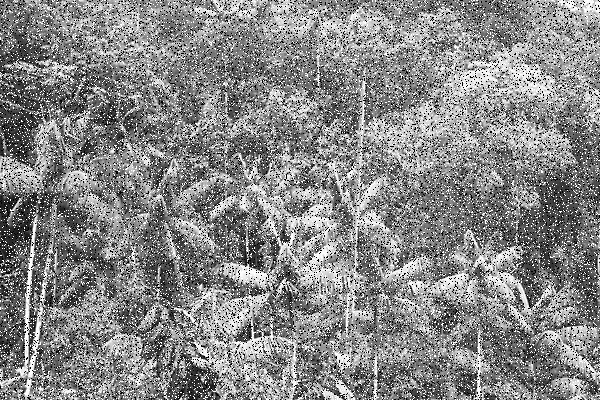
\includegraphics[scale=0.45]{images/Gliese_581d-V2.png}
		Avant

		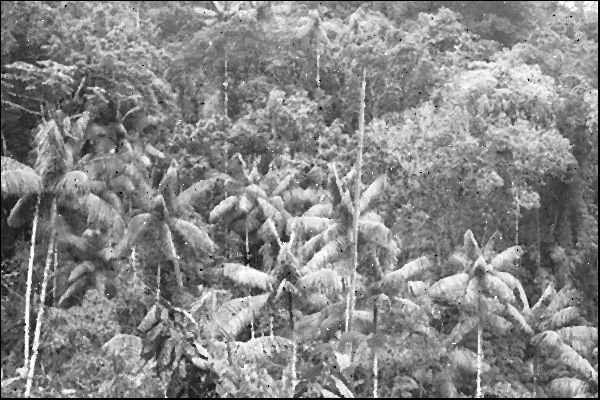
\includegraphics[scale=0.45]{images/MissionX2v2.png}
		Après
		\end{multicols}
	\end{figure}
	\vspace{-0.9cm}

	\paragraph{Procédé}
	\begin{center}
	{\Huge\color{red}A REVOIR}
	\end{center}